\emph{Tekniskt sett kan radioamatörerna världen över, med hjälp av
  sina radiostationer, tämligen lätt skapa kontakt med
  varandra. Därvid krävs att reglerna i de länder som berörs vid
  kontakten respekteras.}

\emph{En hel serie både internationella och nationella regler styr
  radiokommunikationerna i en nation. Varje radioamatör ska känna
  till och följa dessa regler så långt de har anslutning till
  utsträckning harmoniserat sina bestämmelser inbördes.  Nationella
  amatörradio. Vissa länder -- t.ex. CEPT-länderna -- har i någon
  avvikelser förekommer likväl och reglerna i det land, som man gör
  radiosändningar ifrån, ska alltid följas.}

\section{ITU Radioreglemente (RR)}
\index{Internationella Teleunionen (ITU)}
\index{ITU}
\index{ITU RR}
\index{RR}
\index{radioreglemente}
\index{PTS}

Internationella Teleunionen (ITU) är det internationella samarbetsorgan där
olika länders myndigheter (administrationer) för telekommunikation samarbetar
och koordinerar sig, bland annat genom gemensamt regelverk och standarder.
Det är viktigt för att koordinera användning av spektrum och signalerna i det.

ITU Radioreglemente (RR) \cite{ITU-RR} är det övergripande regelverket för att
koordinera spektrum-användning, dvs. för alla former av radio-relaterad
verksamhet. Det är det gemensamma ramverk som används, och där sedan varje land
utgår från det för att sedan skriva de nationella föreskrifterna och
tilldelningarna. Dock, den ansvariga myndigheten behöver inte följa ITU RR
strikt, och det förekommer flera fall där saker i ITU RR ser tillåtna ut men
de nationella föreskrifterna sedan inte tillåter det. Man ska därför inte
tolka ITU RR som det som gäller istället för de nationella föreskrifterna utan
snarare en utgångspunkt. Det kan ha skett förändringar i ITU RR men där
existerande frekvensallokeringar nationellt förhindrar att följa ITU RR.
Omvänt så är det ofta svårt för de nationella föreskrifterna att gå utanför
ITU RR eftersom det kan kräva svåra förhandlingar, och de försöker man ofta
få till i förändringen av ITU RR istället.

I Sverige är det Post- och telestyrelsen (PTS) som är nationell telekommunikation
och spektrum ansvarig, och det är i deras föreskrifter all radio regleras,
inklusive amatörtjänsten. Där ITU RR pratar om administration så avses för
Sveriges del PTS.

Som del av ITU RR definieras ''Amateur services'' \cite[Article 25]{ITU-RR}.
Amatör- och Amatörsatellittjänsterna är radiokommunikationstjänster
med syfte att tillhandahålla nödvändig kommunikation i händelse av
naturkatastrofer, träna operatörer och tekniker i radio- och
telekommunikationsteknik till ingen kostnad för stat och samhälle,
bidra till att tidsenlig radiokommunikation främjas och att förbättra
internationell förståelse och välvilja.

\subsection{Artikel 1 (RR) Termer och definitioner}
\textbf{
HAREC b.\ref{HAREC.c.1.1}\label{myHAREC.c.1.1},
 b.\ref{HAREC.c.1.2}\label{myHAREC.c.1.2}
}
\index{amatörtjänst}
\index{amatörsatellittjänst}
\index{amatörradiostation}
\index{radiostation}

1.56 (RR) \emph{Amatörtjänst} \cite[1.56]{ITU-RR}\\
En radiokommunikationstjänst avsedd för självutbildning, inbördes
kommunikation och tekniska undersökningar bedrivet av amatörer, det
vill säga av behöriga personer intresserade av radioteknik,
endast av personligt intresse och utan ekonomiskt syfte.

1.57 (RR) \emph{Amatörsatellittjänst} \cite[1.57]{ITU-RR}\\
En radiokommunikationstjänst som använder rymdstationer på
jordsatelliter för samma ändamål som för \emph{Amatörradiotjänsten}.

1.96 (RR) \emph{Amatörradiostation} \cite[1.96]{ITU-RR}\\
Radiostation inom \emph{amatörradiotjänst}.

\subsection{Artikel 25 (RR) Amateur services}
\textbf{
HAREC b.\ref{HAREC.c.1.3}\label{myHAREC.c.1.3},
 b.\ref{HAREC.c.1.4}\label{myHAREC.c.1.4}
}

\subsubsection{Sektion I. Amatörtjänst}
25.1 §1 Radiokommunikation mellan amatörstationer i olika länder
skall vara tillåten, om inte administrationen i en av de berörda
nationerna har meddelat att den är emot sådan radiokommunikation.
\cite[25.1]{ITU-RR}

25.2 §2 1) Sändning mellan amatörstationer i olika länder skall vara
begränsad till spontan kommunikation med syftet att nyttja amatörtjänsten,
som definierat i 1.56, och av personlig karaktär.
\cite[25.2]{ITU-RR}

25.2A §2 1A) Sändning mellan amatörstationer i olika länder skall
inte vara kodad med syfte att dölja dess mening, annat än för kontrollsignaler
utbytta mellan jordstation och satellitstation i amatörradiotjänst.
\cite[25.2A]{ITU-RR}

25.3 §2 2) Amatörradiostationer får användas för internationell
radiokommikation för tredje parts räkning enbart vid nöd eller
krishantering.
\cite[25.3]{ITU-RR}

25.5 §3 1) Administrationerna avgör hurvida en person som söker licens
att använda en amatörstation skall bevisa sin förmåga att sända och ta
emot text i morsesignaler.
\cite[25.5]{ITU-RR}

25.6 §3 2) Administrationerna skall kontrollera de handhavandemässiga och
tekniska kvalifikationerna hos varje person som önskar använda en
amatörradiostation. En guide för den kompetens som krävs kan man finna i
senaste upplagan av ITU-R rekommendation M.1544.
\cite[25.6]{ITU-RR}

25.7 §4 Den högsta effekten från en amatörstation skall fastställas
av berörda administrationer.
\cite[25.7]{ITU-RR}

25.8 §5 1) Alla allmänna regler i överenskommelsen och de i denna
artikel skall tillämpas på amatörradiostationer.
\cite[25.8]{ITU-RR}

25.9 §5 2) Under loppet av sändningarna skall amatörstationer sända
sina anropssignaler med korta mellanrum.
\cite[25.9]{ITU-RR}

25.9A §5A Administrationer uppmuntras att vida nödvändiga steg för att
tillåta amatörstationer att förbereda sig för och möta kommunikationsbehov
vid katastroftillstånd.
\cite[25.9A]{ITU-RR}

25.9B §5B En administration kan avgöra hurvida en person som har tillstånd
att använda en amatörstation hos en annan administration kan tillåtas använda
en amatörstation medans denna person befinner sig på tillfälligt besök landet,
samt vilka villkor och begränsningar de väljer att ange.
\cite[25.9B]{ITU-RR}

\subsection{Sektion II. Amatörsatellittjänst}

25.10 §6 Bestämmelserna i Sektion 1 i denna artikel skall gälla i all
tillämplig omfattning även för amatörsatellittjänst.
\cite[25.10]{ITU-RR}

25.10 §7 Administrationer som godkänner rymdstationer i amatörsatellittjänst
ska tillse att tillfredställande jordkontrollstationer upprättas före
uppskjutningen för att säkerställa att varje rapporterad skadlig störning
skall kunna avbrytas omedelbart av den bemyndigande administrationen.
Se 22.1 **.
\cite[25.11]{ITU-RR}

** 22 behandlar ''Space Services''

\subsection{Artikel 5 Frekvenstilldelning}

\subsubsection{Inledning}

5.1 I Unionens alla dokument där termerna \emph{allocation},
\emph{allotment} och \emph{assignment} används skall de ha den
betydelse som ges i 1.16 till 1.18, varvid termerna på de tre
arbetsspråken skall vara som följer (franska, engelska och spanska):
\cite[5.1]{ITU-RR}

Frekvensfördelning till:
\begin{tabular}{lll}
  Tjänster & Allocation & (tilldelning) \\
  Områden & Allotment & (fördelning) \\
  Stationer & Assignment & (anvisning) .... etc. \\
\end{tabular}

(För enkelhetens skull återges här endast betydelserna på engelska språket).

\subsubsection{Sektion I. Regioner och områden}
\textbf{
HAREC b.\ref{HAREC.c.1.5}\label{myHAREC.c.1.5}
}

5.2 För tilldelning av frekvenser har världen delats in i tre
Regioner så som visas på följande karta och som beskrivs i 5.3 till
5.9 .... etc.
\cite[5.2]{ITU-RR}

\emph{ Det innebär att tilldelning, fördelning och anvisning av
  frekvenser mycket väl kan skilja mellan ITU-regionerna. Skillnaderna
  förklaras t.ex. av regionalt olika behovsstruktur, befolkning etc.}

\emph{Det förekommer också likheter. På nedanstående karta har
  markerats en tropisk zon, vilket förklaras av den annorlunda
  vågutbredningen där. T.ex. behöver särskild hänsyn tas vid
  frekvenstilldelning (allokering) till rundradiotjänsten i zonen.}

\begin{figure}
  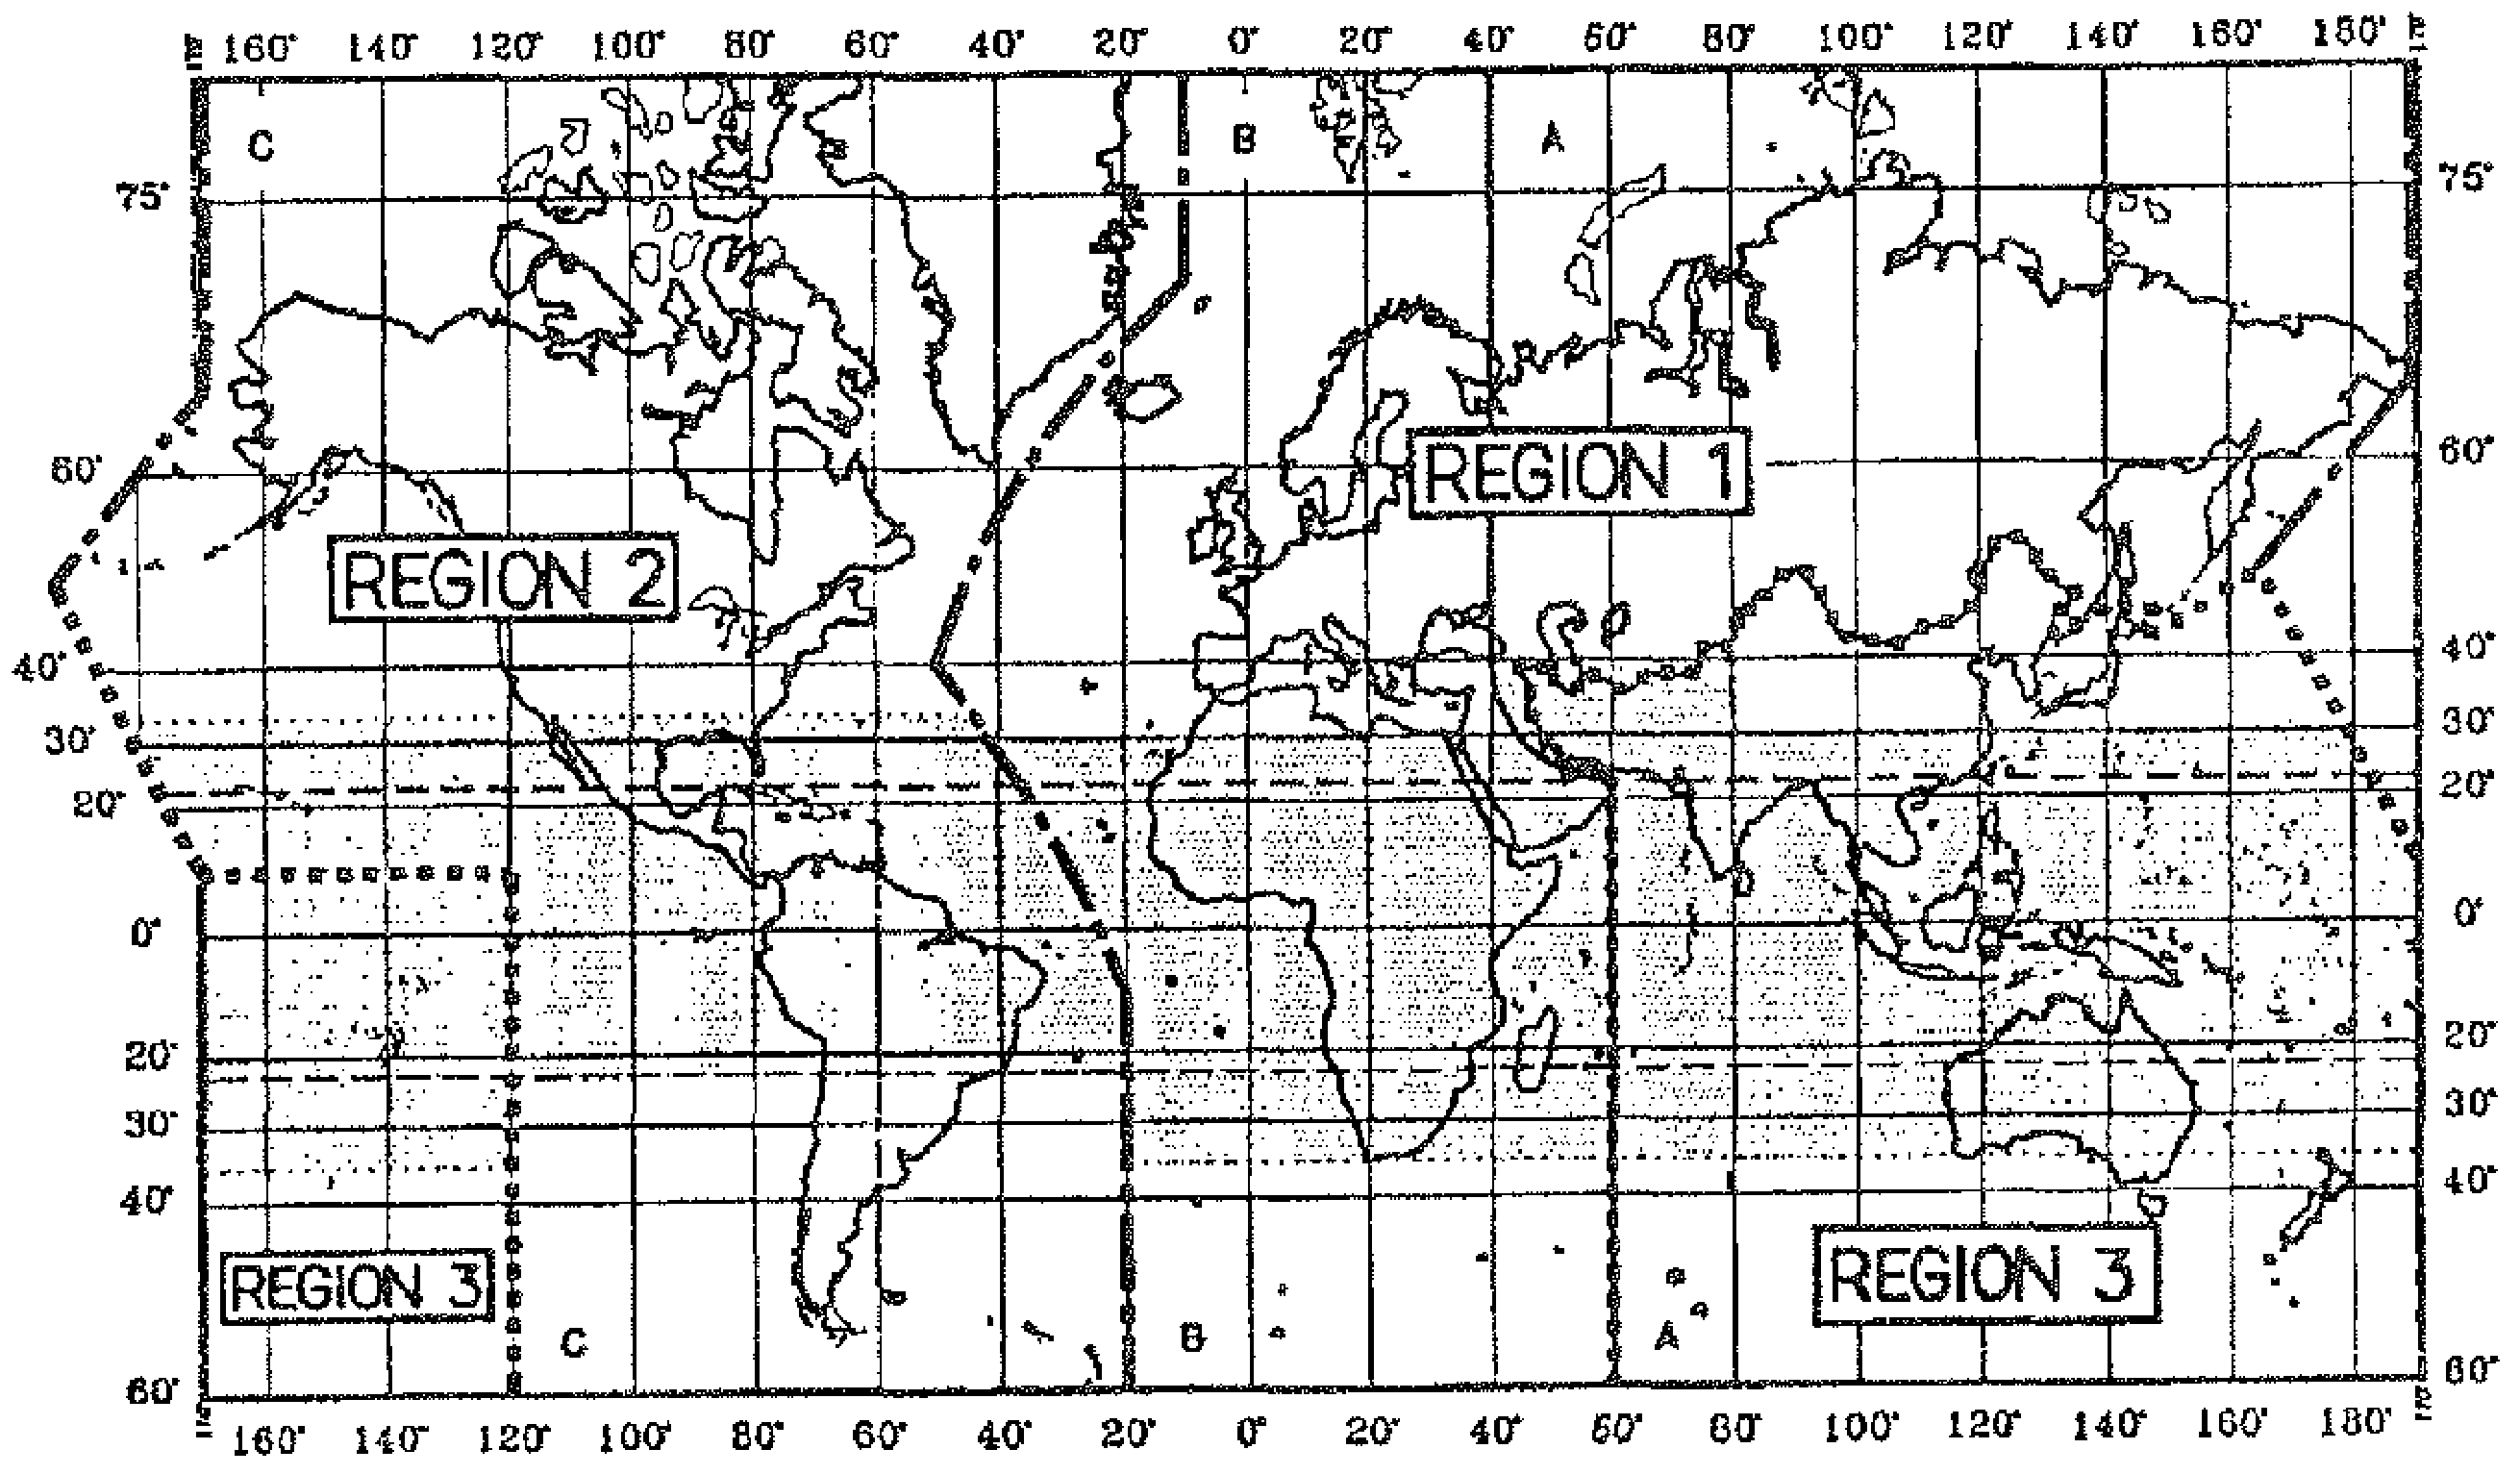
\includegraphics[width=\textwidth]{images/cropped_pdfs/bild_3_2-01.pdf}
  \caption{ITU Regionkarta (ur RRB-2)}
  \label{fig:bildIII2-1}
\end{figure}
